
\begin{section}{Simulation Results}
\label{sec:simulation}

% Need to label states of the state vector in the modeling section [x y v \theta]

The case study investigated in this paper is with a ground vehicle experiencing the effects of sensor and process noise, dynamical changes, while also succumbing to wind disturbances and sensor attacks. The vehicle will be traveling along a pre-planned trajectory with assumed to be known obstacles throughout the environment. (Show a figure, or more, of the vehicle within the environment showing the path and obstacles). We consider a ground vehicle starting at an initial position facing the positive $x$ direction with zero velocity $x(0)=(0,0,0,0)^T$. The objective for the vehicle is to encircle a large object while following a desired trajectory with obstacles of varying distances from the path. During navigation, parameters within the fundamental matrix $\bm{A}(k)$ and input matrix $\bm{B}(k)$ may change by up to 50\%. It is assumed the maximum velocity of the vehicle is 3.0m/s and the desired reference velocity it wants to maintain is 2.5m/s. 


Below is results I will show 
In Figure Xa) the vehicle moving along the trajectory with no compromised sensors and far from obstacles. Velocity is unaltered due to the obstacles being well outside the uncertainty boundaries.

Figure Xb) demonstrates the effects of the loss of a position sensor of low noise profile. The confidence estimation interval has grown in size.

Figure Xc) demonstrates the adaptive motion planner in action when obstacles come within the confidence and uncertainty boundary. Velocity is reduced to shrink both the confidence interval and uncertainty bounds.

Figure Xd) Obstacles are again far away from the given trajectory, outside of the CI and uncertainty bounds. Velocity is restored to desired levels.

Figure Y) displays all sensor measurements for velocity, capturing when the attack occurs and the consequent recovery. 

Figure Z) Showing the detection scheme can decipher the difference between dynamical changes and an attack

% Figure XX) Show convergence of signal to reference

\begin{figure}
\vspace{1pt}
\centering
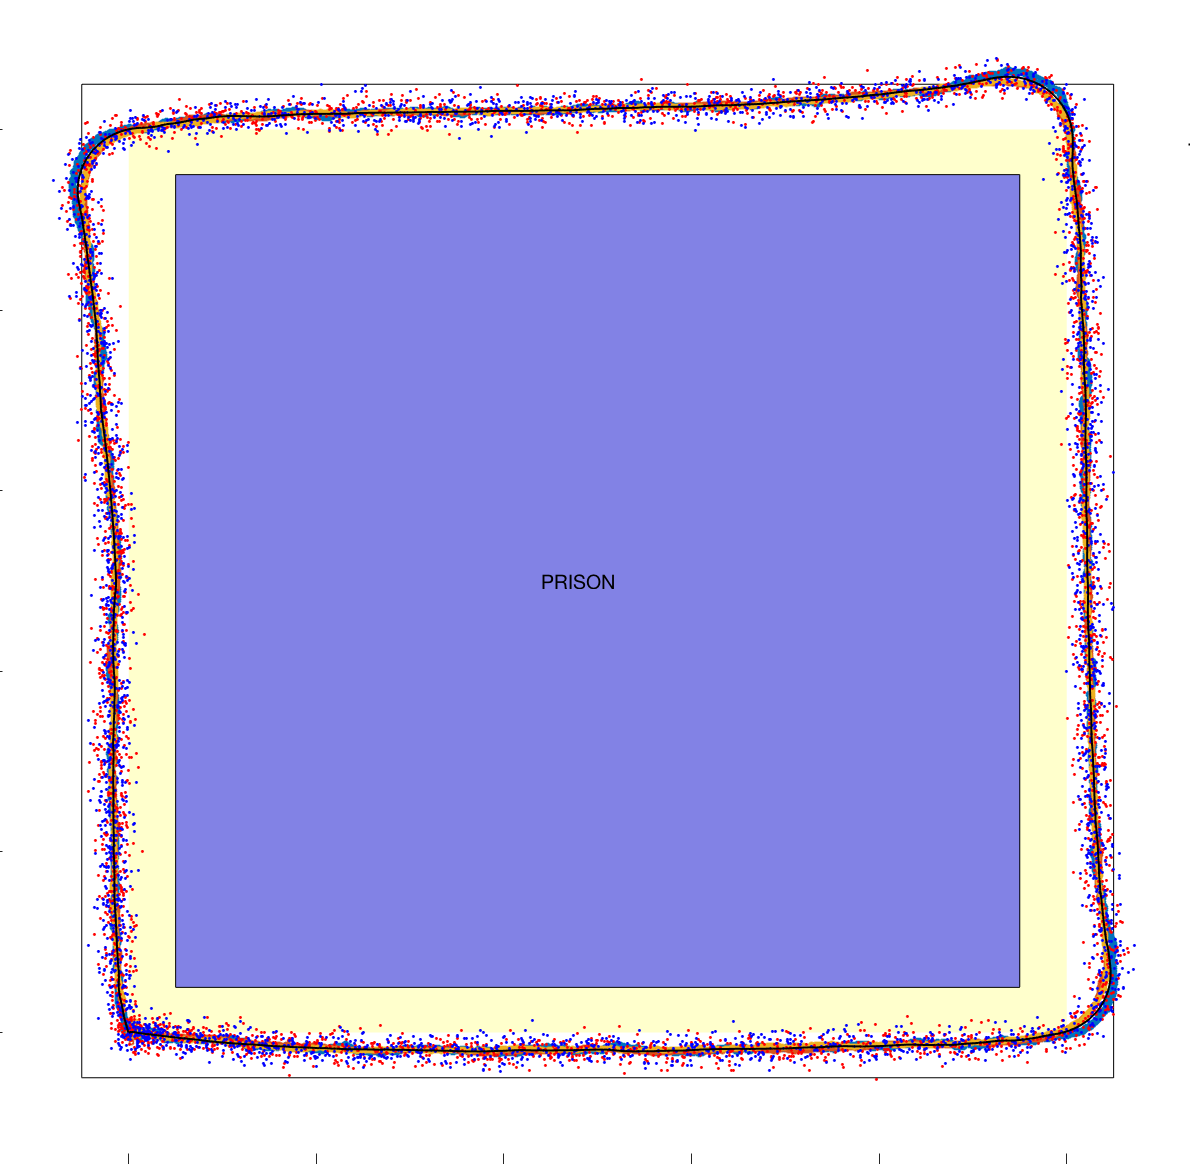
\includegraphics[width=0.48\textwidth]{sim_environment.png}
\caption{The obstacle filled environment the vehicle is traveling through to reach a specified goal point.}
\label{fig:sim_env}
\end{figure}

\begin{figure}
\vspace{1pt}
\centering
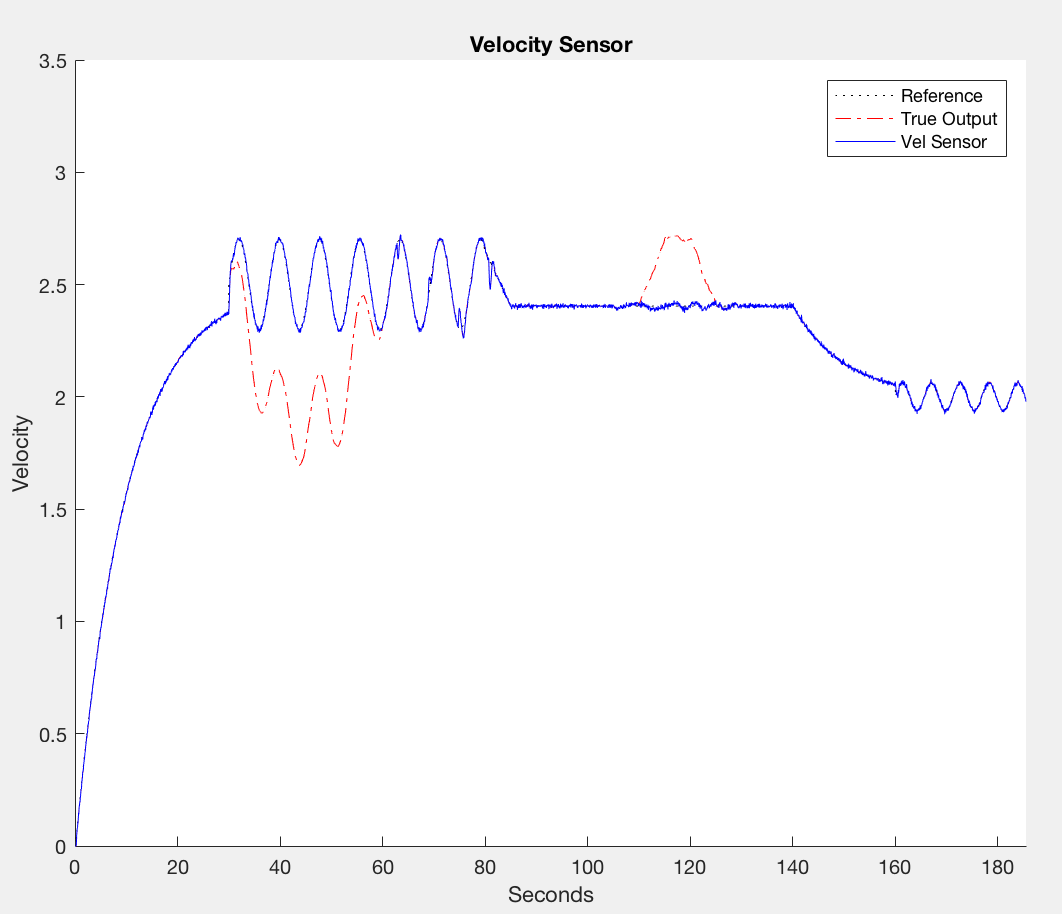
\includegraphics[width=0.48\textwidth]{vel_t.png}
\caption{Vehicle velocity over time exhibiting an attack on a velocity sensor while the system detects and corrects.}
\label{fig:vel_t}
\end{figure}

\begin{figure}
\vspace{1pt}
\centering
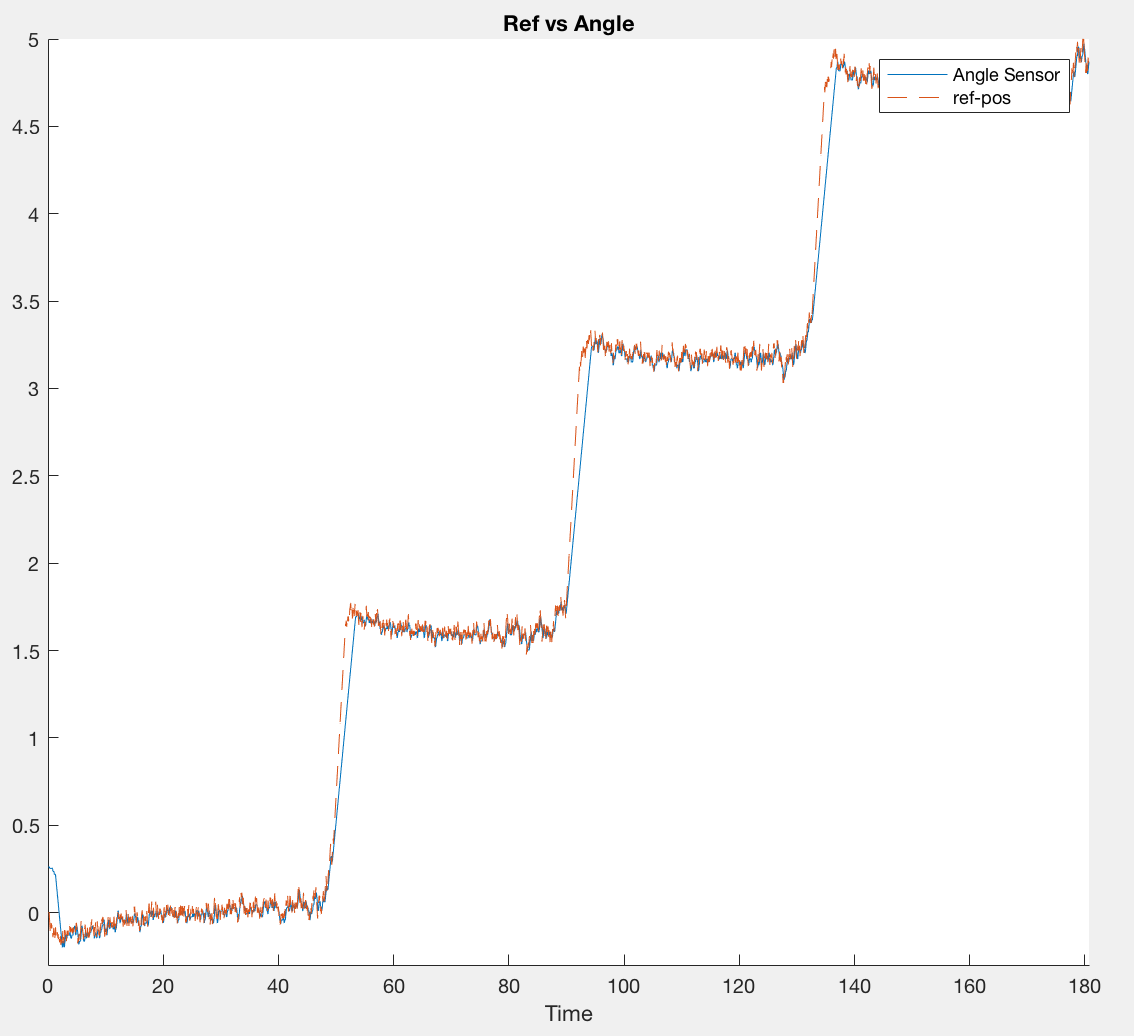
\includegraphics[width=0.48\textwidth]{ang_t.png}
\caption{Vehicle heading angle over time exhibiting an attack on an angle sensor while the system detects and corrects.}
\label{fig:ang_t}
\end{figure}

\end{section}